\title{Raumautomation mit MQTT-Protokoll}

\team{\\
		Gabriel Nussbaumer\\
		Lukas Meienberger}

%\client{Albert Zihlmann}

\coaches{\\
		Albert Zihlmann
}

\fssummary{
	Um den Arbeitsplatz im Büro oder das Wohnzimmer Zuhause angenehmer zu gestalten, gibt es bereits Sonnschutzsysteme, Beleuchtungen, so wie Raumklimageräte. Die IoT-Raumautomation ermöglicht, mithilfe eines kostengünstigen integrierten Systems, die verschiedenen Geräte anzusteuern und einen Überblick über aktuellen Zustand zu haben.
}

\fsgraphics{
	\centering
	\begin{minipage}{1\textwidth}
		\centering
		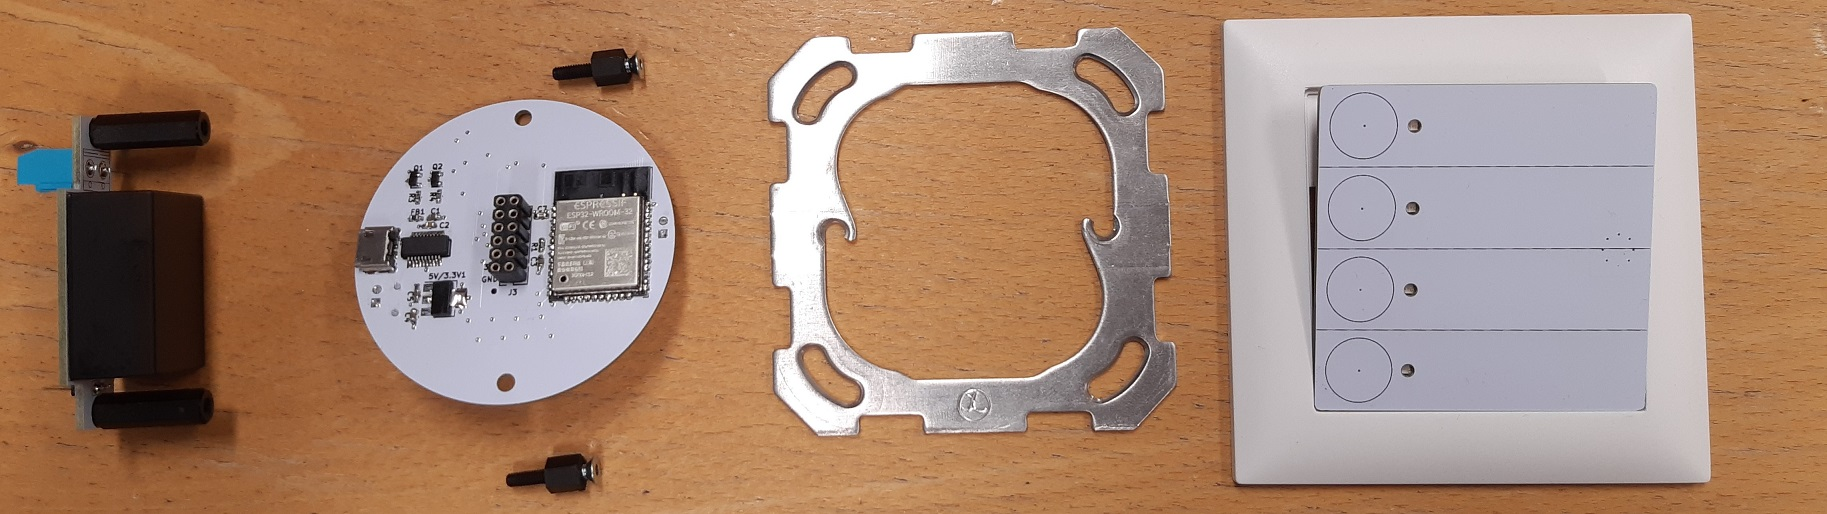
\includegraphics[width=\textwidth]{images/Sensorbaustein_aufbau.jpg}
		\graphicscaption{Der Aufbau des Sensorbausteines}
	\end{minipage}
	\begin{minipage}{0.49\textwidth}
		\centering
		\includegraphics[width=\textwidth]{images/Aktorbaustein_Ansicht.png}
		\graphicscaption{Aktorbaustein}
	\end{minipage}
}

\fscontent{
	\section{Die Aufgabe}
	Die Aufgabe von einer Raumautomation umfasst verschiedene Bereiche und in diesen Bereichen wiederum verschiedene Funktionen. Im Bereich Beleuchtung und Blendschutz übernimmt die Raumautomation die Funktionen von Zeitprogrammen, gerade in Büros, wo es geregelte Anwesenheit gibt. Die Funktion Tageslicht regelt die Beleuchtung so, dass Sonnenlicht genutzt wird und Energiekosten gesenkt werden können. Die Funktion Witterungsschutz verhindert, in Kombination mit einer Wetterstation Schäden an Blendschutzeinrichtungen. Weitere Wetterabhängige Funktionen werden im Bereich Klima genutzt. Die Thermoautomatik Funktion setzt somit der Blendschutz ein, wenn es eine massive Sonneneinstrahlung gibt, und der Raum sich nicht erwärmen sollte.   
	
	
	\section{Handhabung}
	Beim Aufstarten der einzelnen Geräten eröffnet sich ein Accespoint, bei dem mittels Smartphone die Wlan Konfigurationen Durchgeführt werden können. Sobald sich die Geräte ins Lokale Netz verbunden haben, wird automatisch eine Verbindung zum MQTT-Server aufgebaut, der MQTT-Server verwaltet die Nachrichten und managt somit die Kommunikation zwischen den verschiedenen Geräten. 
	
	
	
	\section{Die Lösung}
	Für eine optimale Raumautomation soll eine Plattform auf Basis von einem Aktor- und einem Sensorbaustein erstellt werden.
	Der Sensorbaustein wird dabei ähnlich einer Unterputzsteckdose montiert und hat eine Wlan-Schnittelle, um die Sensordaten auszulesen. Der Anwender wird ein Temperatursensor, ein Touch-Tastenfeld, sowie dazugehörige LEDs, für die
	Interaktion mit dem Baustein zur Verfügung haben.
	Der Aktorbaustein beinhaltet vier Relais und je zwei  0..10 V Aus-/Eingänge.
}

\infobox{Spezifikationen}{%
	
	\hfill
%	\begin{minipage}[t][][b]{0.50\textwidth}\small
		\begin{tabular}{l l l} 
		\textbf{System}&	\textbf{Sensorbaustein}&	\textbf{Aktorbautein} \\
			Kombinierbar&Wlan IEEE 802.11 n&	Wlan IEEE 802.11 n\\ 
			mit KNX, Datenerfassung, &Temperatursensor& 4 x Relais (230 V)\\ 
			in bestehende&Touch-Button& 2 x 0...10 V Eingänge \\ 
			Installationen integrierbar& &2 x 0...10 V Ausgänge \\
	
		\end{tabular} 
%	\end{minipage}
}
